\chapter{Opgaveformulering}
\section{Baggrund}

Virtual- og Augmented- Reality er et af dette års helt store emner. Produkter som HTC Vive og Ocolus Rift har allerede vist hvordan verden kan se ud gennem den virtuelle verden hvor projekter som Google’s Project Tango, Meta 2, og Microsoft’s Hololens i år vil sætte deres præg på augmented reality. Med denne nye teknologi er det op til udviklerne og forbrugerne, at finde ud af hvilke muligheder der kan skabes.
Mange demonstrationer af disse produkter har haft fokus på spil industrien. Her har Microsoft eksempelvis brugt deres Hololens til at se Minecraft fra en helt ny vinkel. HTC har i samarbejde med Steam fokuseret på spil i Steam’s spil univers og flere og flere spil understøtter allerede nu virtual reality. Dette bringer os frem til spørgsmålet, om disse teknologier også ville kunne bruges i en anden kontekst end i spil verdenen. Dette kunne eksempelvis være indenfor retail. Kan en butiksejer bruge teknologien til at sælge sine varer? Hvilket klientel kan benytte sig af den? Og hvad er fordelen ved denne måde at fremstille verdenen på? 

\section{Projekt}
Dette projekt vil have fokus på reklamering og salg ved hjælp af en teknologi der understøtter augmented reality. Vha. Google’s Project Tango vil vi udvikle en applikation, der bruger enhedens front-kamera til at vise virtuelle objekter placeret i den rigtige verden. Objekterne kan være bannere, floor-stickers, papfigurer o. lign. der skal kunne trækkes rundt på enhedens touch-skærm med brugerens fingre. Ydermere foreslår programmet hvor det er mest fordelagtigt at placere objektet henne.
Forslagene fra enheden vil blive basseret på salgsdata fra en samarbejdspartner, der findes i samarbejde med Stibo Accelerator. Udover salgsdata vil vi også fremskaffe people-flow data, der beskriver hvordan kunder bevæger sig rundt i den pågældende butik. Projektet vil også dække arbejdet med denne data. Dvs. hvordan den skaffes, hvorfor den er relevant, og hvordan det bruges. Ud fra dette data forslår enheden den mest fordelagtige placering af objektet. 
Den business intelligence som skal implementeres i produktet, vil blive defineret af hvilken data der kan fremskaffes, stilles til rådighed og hvilken data der er relevant at bruge i denne sammenhæng. Dette betyder at denne data har en stor indflydelse på hvordan det endelige produkt kommer til at agere.
Butiksejere og medarbejdere, der arbejder i større butikker er den primære målgruppe for dette projekt. Her er det muligt at fremskaffe en større mængde data til den business intelligence produktet kommer til at gøre brug af. Herudover kan produktet være med til at skabe et overblik over en butik, hvilket har mere relevans for butikker med mange kvadratmeter kontra butikker med få.

\begin{figure}[H]
\centering
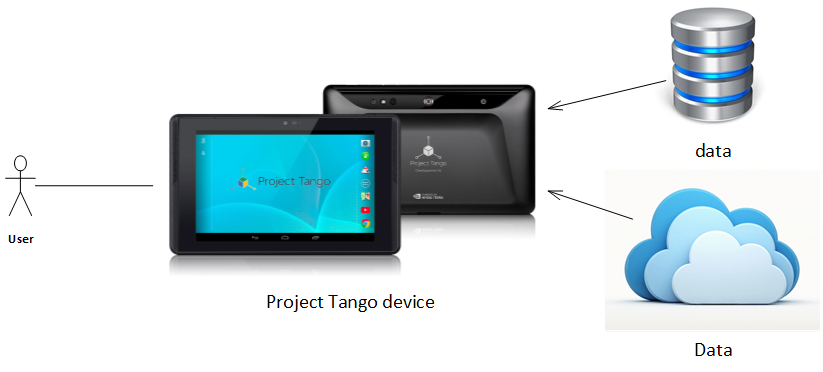
\includegraphics[width=\textwidth]{System_Concept.png}
\caption{Konceptuel produktmodel}
\label{fig:koncept}
\end{figure}


Brugeren vil primært benytte sig af Project Tango enheden, hvor den udviklede applikation ligger på. Den skal modtage data, og evt. processere det, fra eksterne systemer og enheder. Disse eksterne systemer vil ikke blive udviklet i dette projekt, men blive brugt til at definere det endelige produkt.
Et af Projektets formål er at vise at denne nye teknologi ikke udelukkende kan bruges til underholdning, men også kan tilføre værdi til retail verdenen. Da målgruppen for dette produkt ikke kan forventes at have stærke IT-kundskaber, vil der være fokus på at lave et produkt med høj brugervenlighed. 
